%\documentclass{article}
\documentclass[13pt]{ltxdoc}
\usepackage{graphicx}
\usepackage[margin=1.25in]{geometry}
\usepackage[usenames,dvipsnames]{color}
\usepackage{hyperref}
\usepackage{listings}
\usepackage{float}
\usepackage{draftwatermark}
\SetWatermarkText{DRAFT}
\SetWatermarkScale{8}\restylefloat{figure}

\begin{document}

\title{Half-Duplex 10Base-T on an ATtiny85}
\author{Charles Lohr}
%\publicationyear{2014}
%\publicationissue{}
%\publicationmonth{September}
\maketitle



\begin{abstract}
The ATtiny85 Processor by Atmel is an 8-bit RISC microcontroller with 8kB of 
flash, 512 bytes of RAM, and a nominal operating frequency of 20 MHz.
10Base-T Ethernet is an interface standard supported by most modern networking
hardware and enables devices to talk to eachother on a network.  Ordinarily,
specialty hardware is needed to send and receive.  However, by abusing
the USI and PLL and overclocking the ATtiny85 processor, while violating the 802.3 standard, we can communicate to some devices via 10Base-T on a network.
\end{abstract}

\begin{figure}[ht]
    \centering
    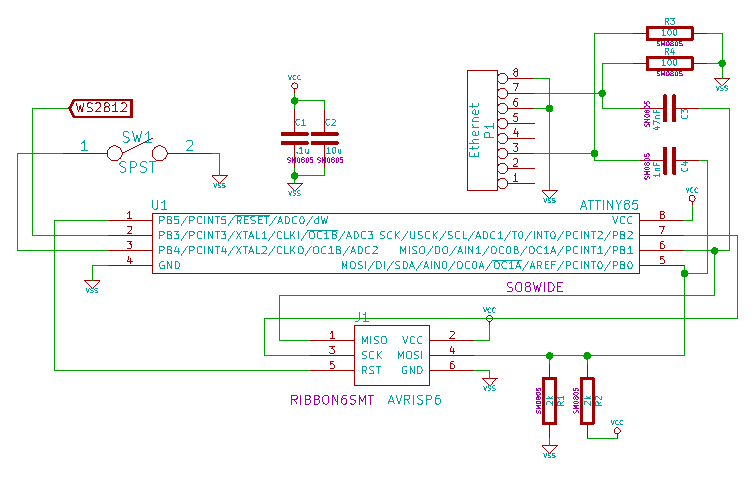
\includegraphics[width=4.2in]{schematic}
    \caption{System Schematic}
	\label{fig:schematic}
\end{figure}

\pagebreak
\section{Introduction}

Although there have been those who have successfully sent packets from an AVR to
the Ethernet on an AVR\footnote{Igor \v{C}e\v{s}ko ``Implementation UDP into microcontroller Igor Atmel-UDP device: UDP/IP infrared remote control'' \url{http://www.cesko.host.sk/IgorPlugUDP/IgorPlug-UDP\%20\%28AVR\%29_eng.htm} (Retrieved Sept 2, 2014)}, their approaches have been limited
to fixed packets with at most one byte of payload changing.  This is not ideal
for a general Ethernet device.

The ATtiny85 processor has a core that operates at one clock cycle per instruction
for most instructions\footnote{Atmel ``8-bit AVR Instruction Set'' 0856D–AVR–08/02 (Retrieved Sept 2, 2014)}.  It has a USI (Universal Serial Interface)
that we can use as a high frequency shift register.  If clocked with Timer 0, 
we can achieve a sample rate of the system clock frequency.  This makes it possible
to send out Manchester-encoded Ethernet frames from RAM when operating at 20 MHz. 

When receiving packets, we need to sample at $\approx$31.5 MHz.  This can be achieved
by using the AVR's internal PLL.  Once the AVR is running above 30 MHz, the USI's 
buffer register is polled.  When an Ethernet frame begins, the AVR can dump the 
bitstream to RAM, and at a later time can decode the Ethernet frame in place.

Our physical interface to the Ethernet is intentionally poor and cheap, as can be seen in
Figure \ref{fig:schematic}.  While
it would be wise in more practical situations to use magnetics and proper termination
even a line driver would be great.  We opted to see what the bare minimum is.

\section{Background}

\subsection{Ethernet Topology}
Ethernet uses a point-to-point communication scheme over separate differential pairs of copper wires, one pair for TX one pair for RX. 
All communication to other devices on the network
is done through the use of switches and hubs.  Switches expect the TX and RX lines to
be opposite that of the client device.  We use the client-style +/- pairs.  If we wish
to connect directly to another client, i.e. a laptop, we would need a crossover or the
other computer would need to support MDIX.

The pairs, TX and RX are differential to aid in common-mode rejection.  Noise
will affect both pairs similarly, and the effective noise on the signal will be minimized.
Additionally, 802.3-2002 mandates all Ethernet devices isolated
the incoming signal to help with noise rejection and prevent ground loop issues, but
most prominently, safety benefits.  \footnote{802.3-2002 Section 14.3.1.1}

While detectable, it generally is not a big deal if the +/- on an individual pair
is swapped.  Our algorithm doesn't care which one is + or -.

Because we ground our signals instead of using magnetics, we will get neither of these
benefits.

\subsection{Manchester Encoding}
Ethernet data is encoded in Manchester encoding at 10 MBits/sec.  Manchester encoding
is a continuous stream that focuses on the changes in bits.

With Manchester decoding, focus is on the location of a rising or falling edge.  Falling 
edges on clock pulses indicate a 0, rising edges indicate a 1.  Manchester guarantees that there
should be approximately as many 1's on the wire as 0's, thus preventing DC offsets.  Figure \ref{manchester}
shows an example Manchester encoded stream.  

This data is transmitted on-wire MSB first.  At any one point in time, it is impossible to
determine if a bit is a 1 or a 0 unless the start-of-message bit is found, as there is no
clock source for Ethernet.  Therefore, it is impossible to know if the signal is falling or
rising on the clock edge.


\begin{figure}
    \centering
    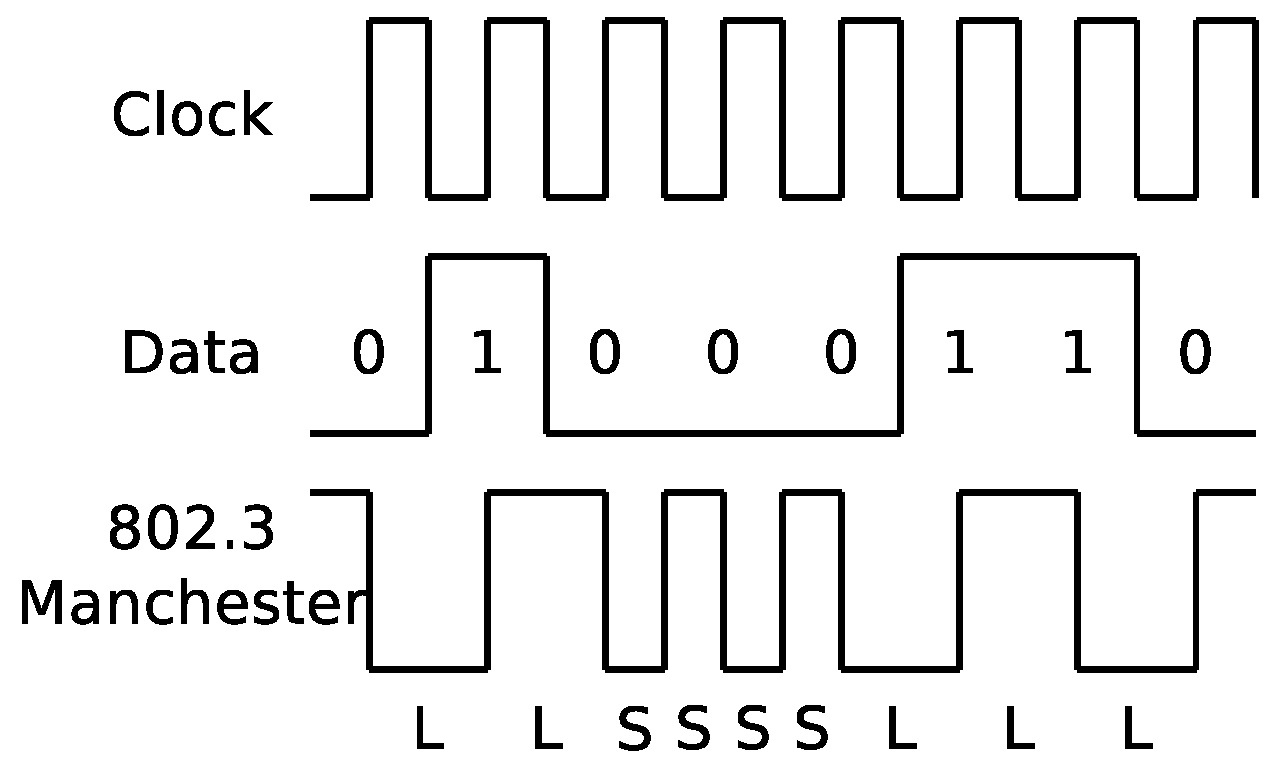
\includegraphics[width=3.0in]{manchester}
    \caption{Manchester Example}
    \label{manchester}
\end{figure}

One way to decode the Manchester if you know what the first bit is, is to look for any long pulses.
Each long pulse indicates a change in bits, and any pairs of short pulses indicate a repeat in bit. 
When the data transitions from a 0 to a 1 or a 1 to a 0, there is a long pulse. For
the section of the packet with many 0's, there are pairs of short pulses.  Making sure that all
short pulses are paired up helps us detect errors early. 

If there are many repeated output 1's or 0's in a row that can mark the end of an Ethernet packet.
While the Ethernet packet is transmitting, there should never be a period when the line is low
or high for longer than .2us.

In order to match up the first bit of the packet, we have to look for the start signature.
Figure \ref{manchesterb} shows what the beginning of the data in an Ethernet packet looks like.
Once we see the pair of 1's, we now know that the packet is starting and can begin 
decoding the packet.

\begin{figure}
    \centering
    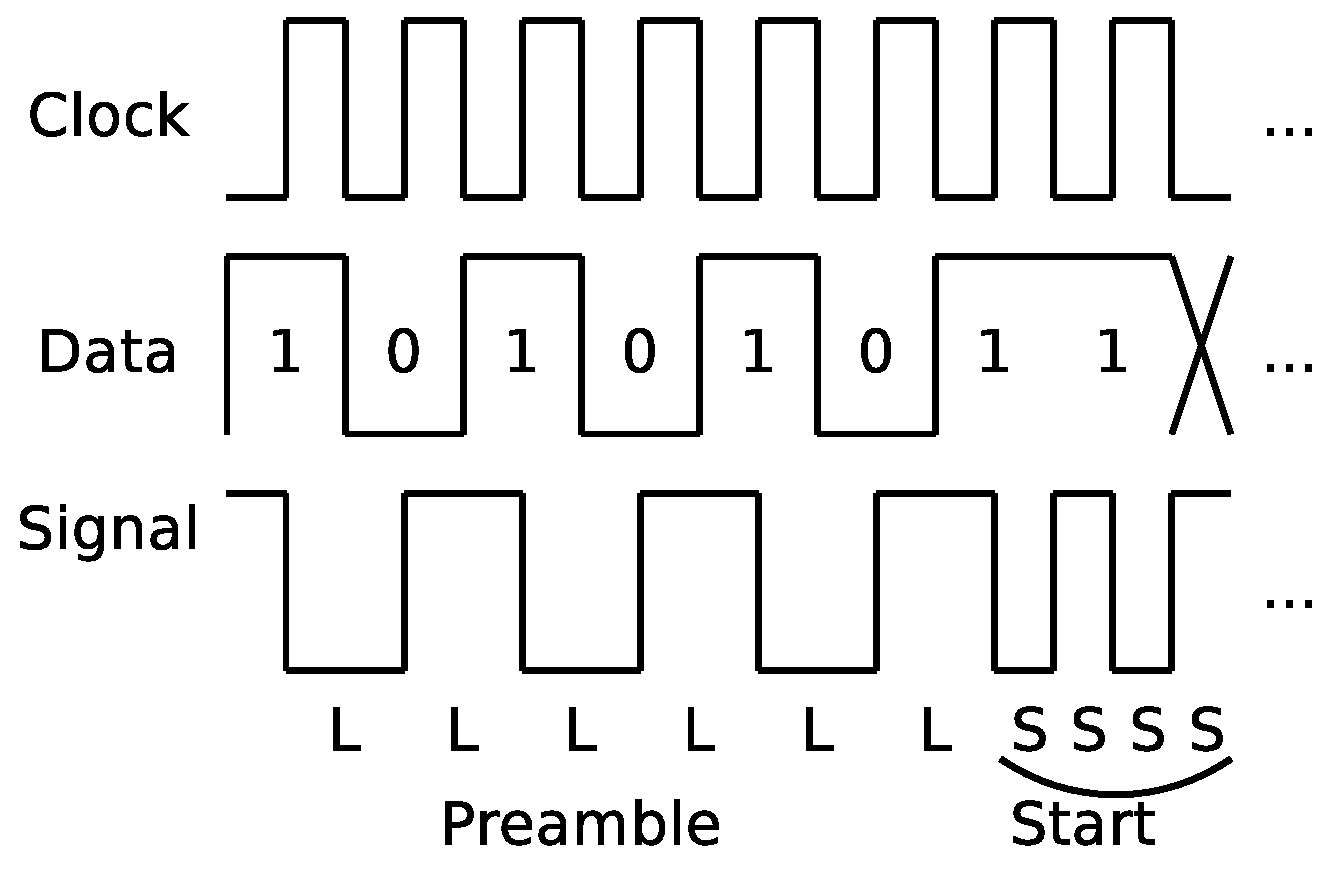
\includegraphics[width=3.0in]{manchesterb}
    \caption{Beginning of frame}
    \label{manchesterb}
\end{figure}


\subsection{IEEE 802.3 Ethernet frame}
The Ethernet frame consists of a preamble, i.e. repeating 0x55's for 7 bytes, with the last
byte being a 0xD5, i.e. the highest bit is flipped to break the chain of alternating low
and high.  This makes it possible for receivers to sync up to the packet at any time during the
preamble.  This can be seen in Figure \ref{manchesterb}.  Practically speaking that gives us $\approx$5uS to begin recording an Ethernet 
before we'll miss the start token and be unable to recover the packet.

Figure \ref{etherfarme} shows us that from there, we have the destination MAC, source MAC, and the rest of our IP packet.
When we're done with the IP Packet, we can have padding so that the frame adds up to 64 bytes, and then at the end, we have an Ethernet CRC.
We had to use a table-less CRC because of the excessive RAM/Flash usage of tabled ones.

\begin{figure}
    \centering
    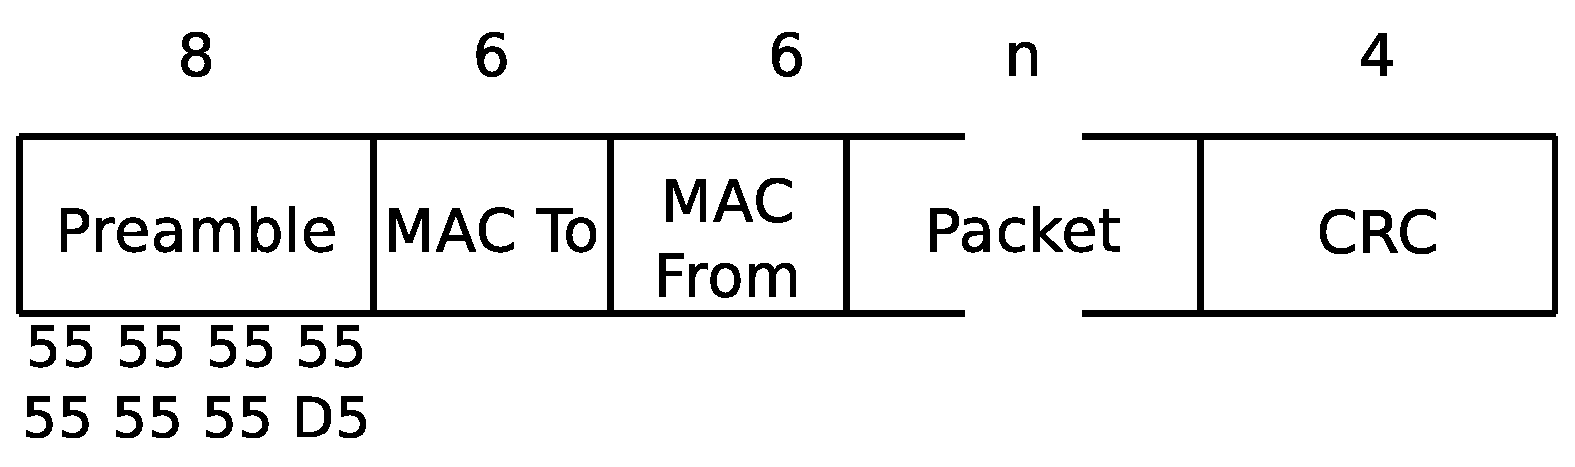
\includegraphics[width=3.0in]{etherframe}
    \caption{Ethernet Packet Example}
    \label{etherfarme}
\end{figure}


\subsection{Link Detection}
Ethernet Links are detected using different autonegotiation schemes depending on speed.  Conveniently,
10Base-T, Half-Duplex is trivial to indicate.  It does not need any codes and simply needs to emit
a new NLP pulse every 16ms that's 100-200ns wide.  This pulse is only in one direction and is not a full
up-and-down.

\section{Hardware}
Figure \ref{fig:schematic} shows the specific schematic we used when developing the software stack.
It is particularly terrible.  It terminates poorly, doesn't have any isolation, doesn't drive very strong (violating the
voltage template) \footnote{IEEE 802.3-2002 Figure 14-9}
and doesn't cleanly receive data.  This is the most minimal set up we were able to use to send and receive packets.

While it worked with short cables (\textless 10 meters) with all hardware we connected it.  When tested \textgreater 10 meters,
to a switch it did not link.

\begin{itemize}
\item C1, C2 are bypass capacitors that maintain power to the chip during brief points where it needs extra power, i.e. transitioning states on the TX pin.
\item P1 is any ethernet connector, it may be female or male.
\item C3 is the TX capacitor.  It develops a 2.5v bias, so the output swing (if no load were applied) would be $\pm$2.5v.
\item C4 is the RX capacitor.  It develops a biased voltage across, so the AVR does not interface with negative voltages.
\item R1, R2 produce a bias in order to raise or lower the DC offset of the incoming signal so that the AVR receives approximately as many 1's as 0's.  It also helps prevent state transitions from being missed entirely.  2k was selected because it happens to have lined up with what I had and worked surprisingly well.
\item R3, R4 are termination resistors, to terminate the signal from the network cable.
\item U1 is the ATtiny85 Processor.
\item J1 is the programming header, compliant with the 6-pin AVR ISP header.
\item WS2812 is any series of WS2812 LEDs.
\item SW1 is a switch.  Because PB4 has an internal pull-up resistor.  This switch will ground that pin.
\end{itemize}

Hardware warnings include:
\begin{itemize}
\item Neither TX nor RX are terminated.  There should be termination resistors.
\item There is no isolation.  There should be magnetics to help to:
\begin{itemize}
\item Reject common-mode noise.
\item Clean up the signal.
\item Add safety to prevent DC transients.
\end{itemize}
\item There is no differential receiver. We are relying on the AVR's Schmitt trigger. \footnote{AVR ATtiny85 Datasheet (2586K-AVR-01/08), Figure 10-2}
\end{itemize}

\section{Software Implementation}
IEEE 802.3 specifies a few different speeds for Ethernet.  One of which that is still
widely supported is 10Base-T, which runs at 10 mbits/sec on-wire transfer - and Ethernet
devices today are still reverse compatible with it.
\textsuperscript{IEEE 802.3 Section 28.1.4}.  We will
mimic a 10Base-T device.  For this we will focus on these aspects:

\begin{itemize}
\item Clocking
\item Use of the USI (Universal Serial Interface)
\item Normal Link Pulses (NLP)
\item Transmitting Manchester encoded packets
\item Receiving Manchester encoded packets
\item Overall process.
\end{itemize}

All source code is available on github in the "ethertiny" project.  At the time
of initially writing this paper, all code for this paper was in the "t85spi" folder.

\subsection{Clock}
We opted to
use the USI on the ATtiny85, clocked at the system clock.  This enables us to
write one byte at a time that will be shifted out of the USI over the next eight
clock cycles.  This gives us enough time to Manchester encode bytes of Ethernet
traffic in RAM on-the-fly.  This is good because it means we do not need to pre-
process the packet and we do not need to use extra RAM to store it.

In order to obtain 20 MHz, we arbitrarily picked an OSCCAL value of 0xbb on our
hardware.  Although this should change from chip to chip, we've found that in most
cases, surprisingly, this value seems to hold.  Additionally, we have to configure
the clock fuses to CKSEL=1.  Our fuses for this are found in Listing \ref{lst:avrdude_fuses}.
Default EFUSEs and HFUSEs are acceptable.  We also enable PLLE and PCKE for any additional
hardware as seen in Listing \ref{lst:clkcmd}.

\begin{figure}
\begin{lstlisting}[caption=AVRDude Fuse Command Line\label{lst:avrdude_fuses},, frame=single]
avrdude -c usbtiny -p t85 -U lfuse:w:0x41:m
\end{lstlisting}
\end{figure}

\begin{figure}
\begin{lstlisting}[caption=Clock Setup\label{lst:clkcmd},language=C, frame=single]
PLLCSR = _BV(PLLE) | _BV( PCKE );
OSCCAL = OSC20;
\end{lstlisting}
\end{figure}


To move to $\approx$31.5 MHz for receiving, we simply set OSCCAL to 0xff.  Once done, we move it back to 0xbb for all other operations.

\subsection{USI}
The USI on the ATtiny must be clocked at the system clock in order to input and output the data fast enough.
To do this, we configure Timer 0 to clock at the system clock rate in CTC mode, with a "top" time of 0.
Provided we operate on it every eight clock cycles, we can create or read
a continuous stream of 1's and 0's at the clock rate.

Listing \ref{lst:usisetup} shows the code to activate Timer 0 and configure the USI to use it. 
When reading from the USI, it is important to use the USIBR.  When writing to it, it is important to use the USIDR.

We have to keep the USI disabled when not in use.  If we leave it enabled, data coming in will be shifted through.  
That means that whenever the USI is enabled, we must be constantly filling the incoming buffer or reading the buffer.
We do not want the incoming data from the network to be shifted back out.  It is convenient to leave the USICR setup and then
set the flag to enable it once we're ready to load in new data and go.


\begin{figure}
\begin{lstlisting}[caption=USI Setup\label{lst:usisetup},language=C, frame=single]
//Setup timer 0 to speed along.
//Timer 0 will be dedicated.
TCCR0A = _BV(WGM01); //CTC mode.
TCCR0B = _BV(CS00);  //Use system clock with no divisor.
OCR0A = 0;

USICR = _BV(USIWM0) | _BV(USICS0) |
	_BV(USITC);

//setup port B
PORTB &= ~_BV(0); 
DDRB &= ~_BV(0);
PORTB &= ~_BV(1);
USICR &= ~_BV(USIWM0);  //Disable USICR

DDRB |= _BV(1);

//Optional, changes bias.
//PORTB |= _BV(0);
\end{lstlisting}
\end{figure}


\subsection{NLPs}
10Base-T Ethernet uses link pulses, or a single up-going pulse that lasts 10-20us
every 16ms $\pm$ 8ms \textsuperscript{IEEE802.3 Section 14.2.1.1}.  This is used to tell
the connected Ethernet device that this device is here, that it's alive, and that it's a
10Base-T, Half-duplex device.  Instead of using the USI on the AVR to create this
signal, we opt to manually turn the pin on and off at the correct times in
Listing \ref{lst:nlp_code}.  Provided the USI is turned off, DDRB is configured as
an output, and we're operating at 20 MHz.  This will produce a $\approx$.15us pulse.

\begin{figure}
\begin{lstlisting}[caption=NLP Code\label{lst:nlp_code},language=C, frame=single]
PORTB |= _BV(1);  //2 cycles
NOOP;  //1 cycle
PORTB &=~_BV(1);  //2 cycles
\end{lstlisting}
\end{figure}

\subsection{TX Manchester-encoded packets}
When operating at 20 MHz, it would be possible to manually bit-bang out a message
via two GPIOs.  If we do that, we also get the added bonus of differential
signaling.  However, if we do this, then there is very little room to modify
the packet.  In fact, we would only be able to modify at most one byte and a
few bits.


\begin{figure}
\begin{lstlisting}[caption=Manchester Lookup Table\label{lst:mantable},language=C, frame=single]
char ManchesterTable[16] __attribute__
	((aligned (16))) = {
	0b10101010, 0b01101010,
	0b10011010, 0b01011010,
	0b10100110, 0b01100110,
	0b10010110, 0b01010110,
	0b10101001, 0b01101001,
	0b10011001, 0b01011001,
	0b10100101, 0b01100101,
	0b10010101, 0b01010101,
};
\end{lstlisting}
\end{figure}

We can store a pre-computed Manchester, Listing \ref{lst:mantable} table for each possible nibble of output
and look up into that table while we're shifting the data out.  In that table, the data in address
0 represents the data that would need to be shifted out to represent a binary 0000, the value in address
address 13 ``d'' (1011 binary), is 01100101, pattern we saw in Figure \ref{manchesterb}.  The reason for the alignment
is because the bottom nibble of its address must be 0x0, so we can use bitwise operations to look up
into the table.

The function that handles sending packets is SendTestASM, and it is written in assembler for the AVR as
to tightly control the timing of writing to the USIDR register.  Figure \ref{sendexplain} shows the progression
of a transmit operation. We first
read the byte we want to send out of RAM, look at its bottom nibble, look that up in the Manchester
table, send the bottom nibble's  Manchester, read the high nibble, look it up in the Manchester table, and
send that.  Then, we look at the next byte and do the same, all in groups of 4 bytes.

\begin{figure}
    \centering
    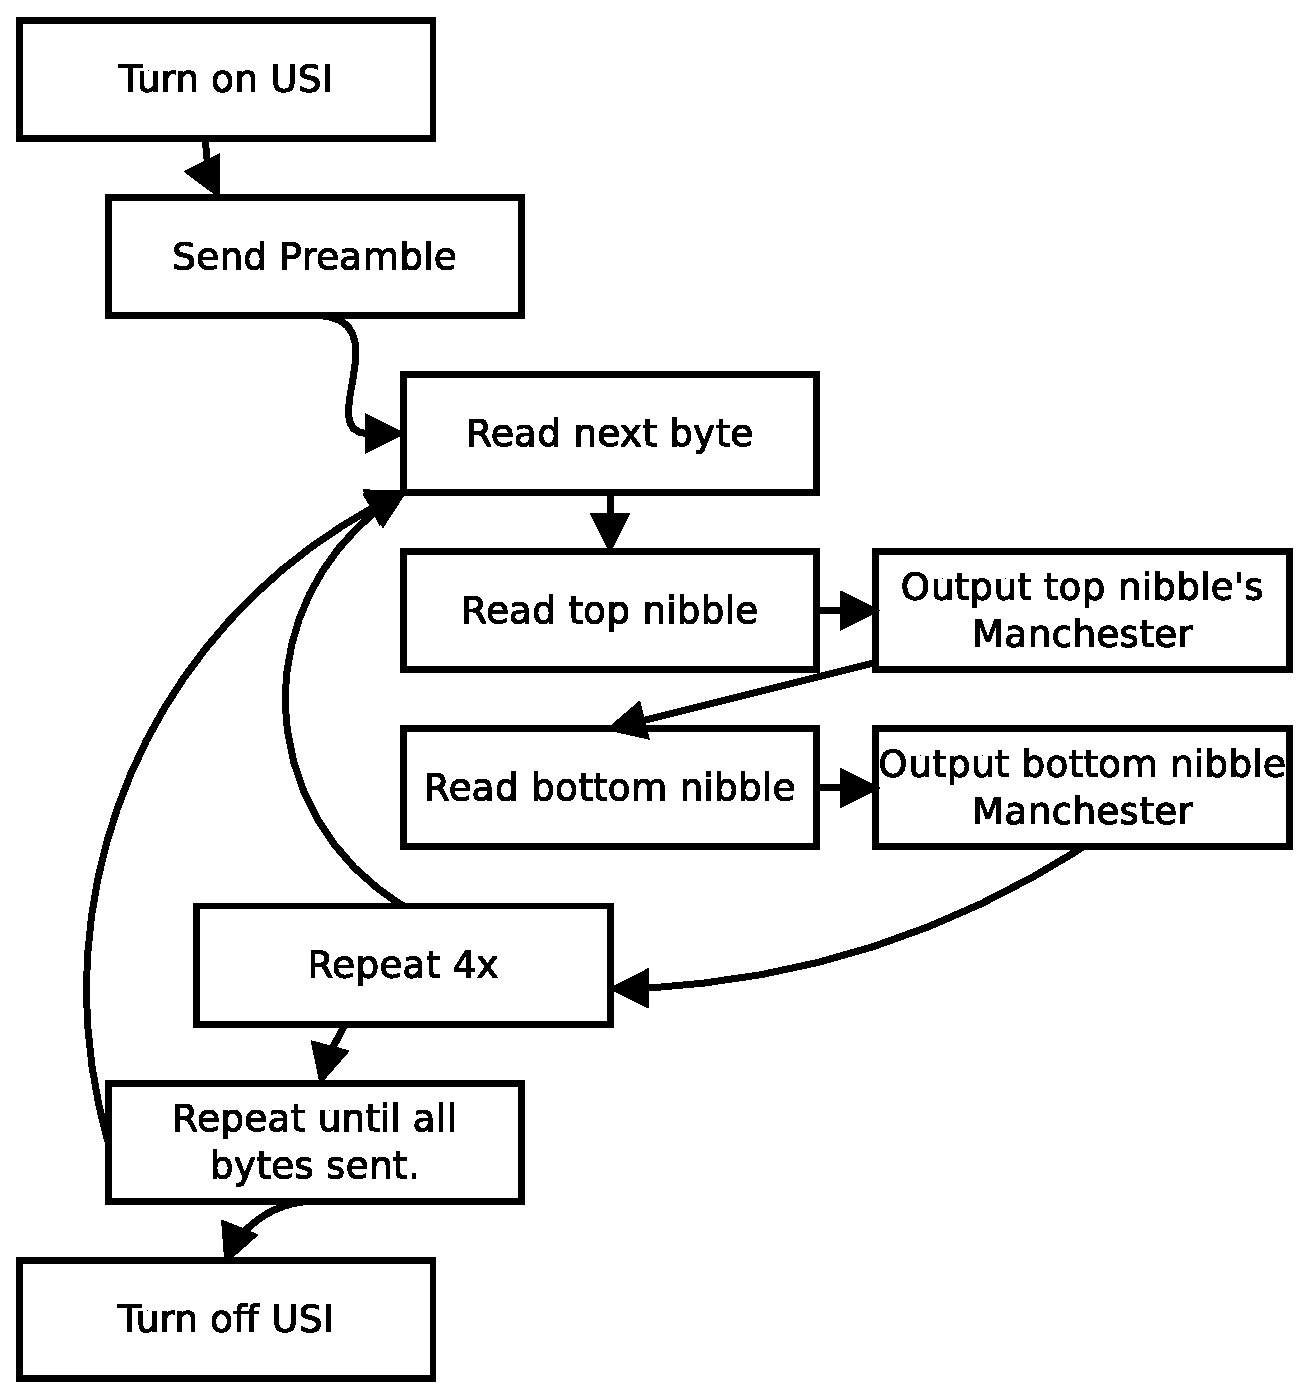
\includegraphics[width=3.0in]{sendexplain}
    \caption{High-level SendTestASM}
    \label{sendexplain}
\end{figure}

Unfortunately, in order to actually accomplish this, we have to heavily interleave the code.  The 
reason we must interleave the code is some operations such as checking to see if we are done with
sending all of the bytes take three operations, and there is only one free operation every time
we send another byte.  By sending groups of four bytes, that extra free cycle we gain per-byte can build up so we can
do our three-cycle compare and jump at the end.  

\subsection{RX Manchester-encoded packets}
Doing the Manchester decoding is the difficult part.  Without using external hardware to lock onto
the loop, or to detect the phase, it means we have to do that entirely with the AVR.  Because it is
also difficult to tweak the AVR's clock to get in phase with the Ethernet signal, we opted to 
stream the bits in software.

Manchester encoding can be decoded entirely in software with a sample rate that exceeds three
times the symbol rate.  That would means our AVR would have to run above 30 MHz, which
conveniently is possible.

By sampling at three times the rate, we can identify ``Long'' and ``Short'' transitions.  Additionally,
the fact that a signal is a ``1'' or a ``0'', incoming becomes irrelevant, and we can focus only on
the transitions.  In order to read in the data, we operate in much the same way we TX'ed the packet.  However
we need to wait for a reading from USIBR that is not 0x00 or 0xff, i.e. it contains both 1 and 0 bits. That
would mean we likely have a packet.

Once we see that change, provided we're operating at $\approx$31.5 MHz, we can begin to capture the packet
by continuously reading USIBR every eight cycles.  After every two packets, we can check to see if
it is all 1's or all 0's.  If it is, we can stop, if not, we continue to capture to RAM.

To understand how we can go from a Manchester bitstream to a series of 1's and 0's, we first
have to understand how we can determine the difference between short and long transitions.  Figure
\ref{demanchester} shows this conversion in the creation of the ``counts'' row from the ``values'' row.
Once we have them, we can pair the shorts together and identify whether bits are flipping or not.

Considering that we can look for the start of packet flag, the 0xD5 from the beginning, we can maintain
whether the current bit is a 0 or a 1 throughout the life of the packet.

\begin{figure}
    \label{demanchester}
    \centering
    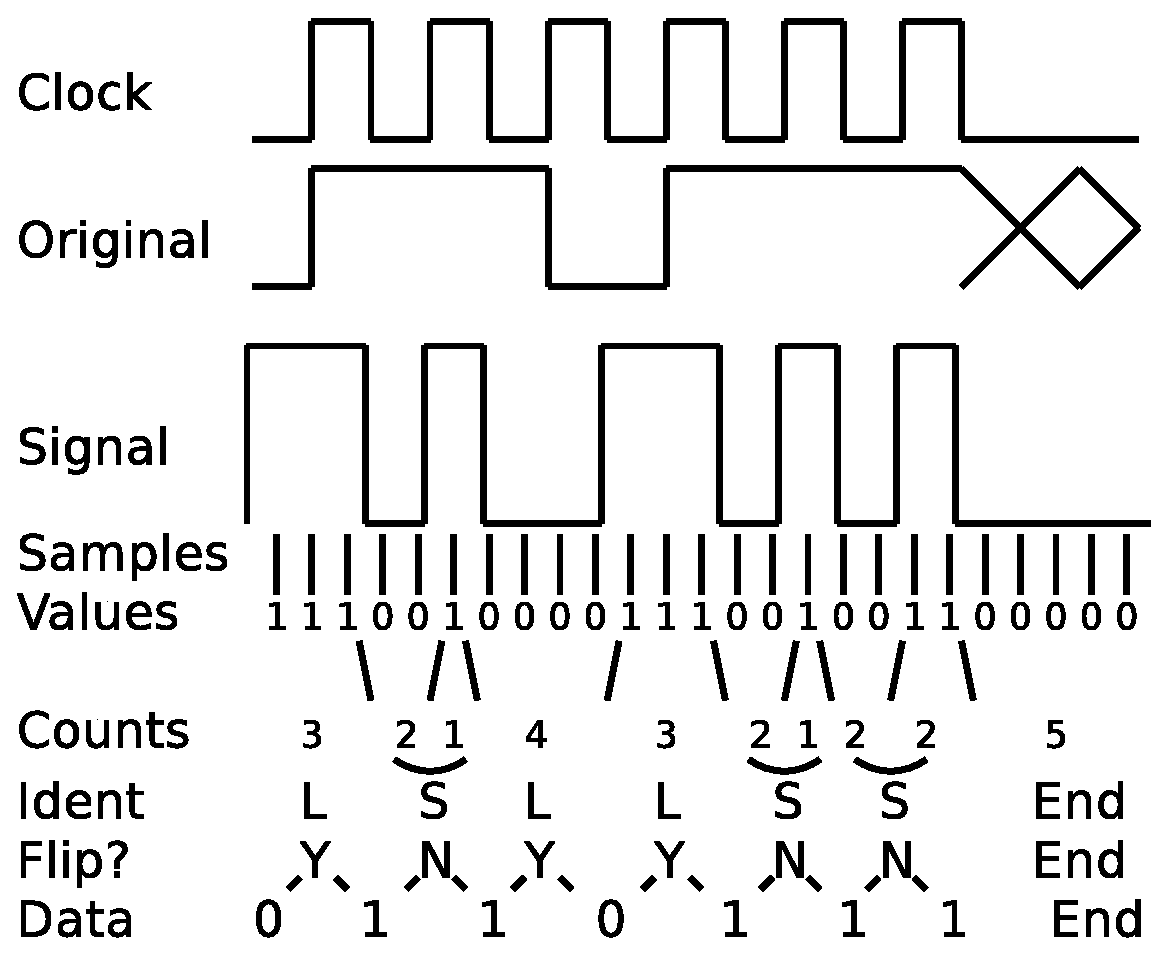
\includegraphics[width=3.0in]{demanchester}
    \caption{Demanchestration (33 MHz clock)}
\end{figure}

A copy of the Demanchestrate function can be found in the code tree in \texttt{hlprocess.c}.

It is important to note that Demanchestrating the packet can be done in-place.  It is
safe to overwrite the raw data with the packet as it is decoded because the packet is always shorter
than the raw data coming in.

Once a packet is decoded, provided there are no bit errors, i.e. unmatched shorts, or missed
shorts, we can begin the CRC \footnote{CRC Code from: http://www.hackersdelight.org/hdcodetxt/crc.c.txt}.  We can use the same CRC that we use for sending in order to verify that the packet
was received successfully.

From there, we can pass it to the IP stack, where it will deal with the packet.  An IP 
stack is outside the scope of this document.

\subsection{Overall Process}
We have covered how we can set up the system, how we can send NLPs, and how we can send and receive
packets. In order to make this work, we put it in a main loop.

We wait for packets for 8ms, send an NLP, wait for more packets for 8ms, do whatever housekeeping work we want, and then repeat the process.

\section{Conclusion}
We have been able to implement a UDP/IP stack with ARP, UDP, and ICMP on an attiny85.  We have tested it
with short wire runs to a few different types of switches and computers and found that we could communicate.
We can send and receive packets up to a $\approx$90-bytes on-wire or 48-bytes of UDP payload.
We have had very high packet loss, on the order of 10-30 \% of the packets.  This is important
when considering applications for this technology, as all protocols the user would have to use must be
robust, able to handle lost packets gracefully, and must not be CPU intensive.

Additionally, because the stack takes a considerable amount of RAM, very little RAM is left over for user
applications unless the user decides to tune back the stack's buffer - which would further limit the 
maximum packet size.

When operating at full speed, our stack uses $\approx$25 mA at 4.5v - less than 1/8 of a watt.

Though impractical for most applications, this stack may prove useful in niche applications where 
cost, power size or other factors outweigh robustness, transfer speeds, or reliability.

\section{Future Work}
We could do a number of things from here that would be useful and interesting.  A few are listed below:

\begin{itemize}
\item Use T0 input from PLL PWM on the AVR to increase sampling rate to 35 MHz, to improve input performance.
\item Synchronize use of USIDR / USIBR to verify the AVR will not encounter a conflict with the shift register.
\item Use a differential driver/receiver to drive the actual signal.
\item Use the internal pull-up to tune the bias, detect if this pull-up helps somehow.
\item Optimize the Demanchestration function in assembly.
\item Use interrupts to send NLPs.
\item Use interrupts to trigger receives.
\item Automatically calibrate the proper OSCCAL for sending based on incoming packets.
\item Improve error correction based on matching pairs and long/short segments. (Improvements to the Demanchestrate function)
\end{itemize}


\end{document}

